\setAuthor{Tundmatu autor}
\setRound{lahtine}
\setYear{2005}
\setNumber{G 2}
\setDifficulty{2}
\setTopic{Dünaamika}

\prob{Tõus}
Talvise ilmaga Tartust Tallinnasse sõitev auto peab oma teekonna alguses ületama järsu ja libeda tõusu Jakobi tänaval (vt joonist). Tõusu kallak horisontaalsihi suhtes $\alpha \approx \ang{5}$, pikkus $l \approx \SI{200}{m}$. Hinnata, kui suur on minimaalne hõõrdetegur $\mu$ rataste ja tee vahel, mille puhul kiirusega $v = \SI{30}{km/h}$ mäkke üles sõitma hakkanud auto suudab veel tõusu ületada?

\begin{center}
	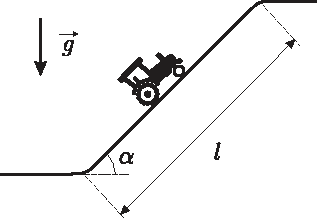
\includegraphics[width=0.5\linewidth]{2005-lahg-02-yl}
\end{center}

\hint
Mäe tippu jõudmiseks peab esialgne kineetiline energia olema suurem kui hõõrdejõu ja raskusjõu ületamiseks vajalik töö.

\solu
Autole mõjuv veojõud on määratud tee ja rataste vahelise hõõrdeteguriga. Antud juhul hõõrdumine ei takista liikumist, vaid, vastupidi, on liikumise aluseks. Kui hõõrdetegur oleks võrdne nulliga, siis ei saaks auto üldse edasi liikuda. Kanname joonisele kõik autole mõjuvad jõud (vt joonist): raskusjõu $F_r = mg$, toereaktsiooni $N = mg \cos \alpha$ ja hõõrdejõuga võrdse veojõu $F_v = \mu mg \cos \alpha$.

\begin{center}
	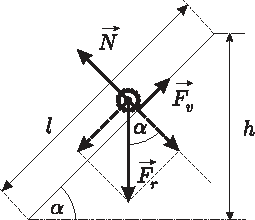
\includegraphics[width=0.5\linewidth]{2005-lahg-02-lah}
\end{center}

Paneme kirja energia miinimumitingimuse mäkke tõusu jaoks:
\[
E_h = E_0 + A,
\]
kus $E_h = mgh = mgl\sin \alpha$ on auto potentsiaalne energia mäe tipus, $E_0 = mv^2/2$ on auto kineetiline energia mäe jalamil ning $A = F_vl = \mu mgl \cos \alpha$ on auto mäkke vedamiseks hõõrdejõu poolt tehtud töö. Saame
\[
m g l \sin \alpha=\frac{m v^{2}}{2}+\mu m g l \cos \alpha.
\]
Sellest võrrandist saame avaldada otsitava hõõrdeteguri:
\[
\mu=\tan \alpha-\frac{v^{2}}{2 g l \cos \alpha}=\tan \ang{5}-\frac{(\num{30} \cdot \num{1000} / \num{3600})^{2}}{\num{2} \cdot \num{9,8} \cdot \num{200} \cdot \cos \ang{5}} \approx \num{0,07}.
\]
Arvestades, et libedal jääl võib hõõrdetegur langeda alla \num{0,05}, võib meie auto teoreetiliselt koju jääda, kui tee on libe ja teele pole õigeaegselt liiva pandud ning autol pole naastrehve all.
\probend